\chapter{Universal software for machine learning in regulatory genomics}
\label{chap:chapter 1}

%%%%%%%%%%%%%%%%%%%%%%%%%%%%%%%%%%%%%%%%%%%%%%%%%%%%%%%%%%%%%%%%%%%%%%%%%%%%%%%%
\section{Abstract}
%%%%%%%%%%%%%%%%%%%%%%%%%%%%%%%%%%%%%%%%%%%%%%%%%%%%%%%%%%%%%%%%%%%%%%%%%%%%%%%%

Deep learning (DL) has become a popular tool to study cis-regulatory function. Yet, efforts to design software for DL analyses in regulatory genomics that are Findable, Accessible, Interoperable and Reusable (FAIR) have fallen short of fully meeting these criteria. Here, we present EUGENe (Elucidating the Utility of Genomic Elements with Neural Nets), a FAIR toolkit for the analysis of genomic sequences with DL. EUGENe consists of a set of modules and subpackages for executing the key functionality of a genomics DL workflow: 1) extracting, transforming and loading sequence data from many common file formats, 2) instantiating, initializing and training diverse model architectures, and 3) evaluating and interpreting model behavior. We designed EUGENe as a simple, flexible and extensible interface for streamlining and customizing end-to-end DL sequence analyses, and illustrate these principles through application of the toolkit to three predictive modeling tasks. We hope that EUGENe represents a springboard toward a collaborative ecosystem for DL applications in genomics research.

%%%%%%%%%%%%%%%%%%%%%%%%%%%%%%%%%%%%%%%%%%%%%%%%%%%%%%%%%%%%%%%%%%%%%%%%%%%%%%%%
\section{Main}
%%%%%%%%%%%%%%%%%%%%%%%%%%%%%%%%%%%%%%%%%%%%%%%%%%%%%%%%%%%%%%%%%%%%%%%%%%%%%%%%

Cracking the cis-regulatory code that governs gene expression remains a fundamental challenge in genomics research. Efforts to annotate the genome with functional genomics data\cite{ENCODE_Project_Consortium2012-tn} have powered machine learning methods that aim to learn biologically relevant sequence features by directly predicting these readouts. Deep learning (DL) has become especially popular in this space, and has been successfully applied to tasks such as DNA and RNA protein binding motif detection\cite{Alipanahi2015-ef,Pan2018-of,Quang2019-gi,Koo2021-ly,Wang2018-ls}, chromatin state prediction\cite{Zhou2015-rk,Quang2016-ll,Kelley2016-oh,Kelley2018-if,Minnoye2020-vz,Atak2021-sz,Li2021-sb,Yuan2022-gg,Chen2022-bn,Janssens2022-vy,Nair2019-um,Ullah2021-th}, transcriptional activity prediction\cite{Kelley2018-if,Zhou2018-mt,Agarwal2020-os,Avsec2021-hh,Karbalayghareh2022-gt} and 3D contact prediction\cite{Fudenberg2020-gs,Zhou2022-mp,Yang2021-yq,Tan2023-ro}. Recently, complementary models have been developed to predict data from massively parallel reporter assays (MPRAs) that directly test the gene regulatory potential of selected sequences\cite{De_Almeida2022-aa,Movva2019-jo,Jores2021-iu}. Most encouragingly, many of these multilayered models go beyond state of the art (SOTA) predictive performance to generate expressive representations of the underlying sequence that can be interpreted to better understand the cis-regulatory code\cite{Avsec2021-sw,Janssens2022-vy,De_Almeida2022-aa}.

Despite these advances, executing a deep learning workflow in genomics remains a considerable challenge. Though model training has been substantially simplified by dedicated DL libraries such as PyTorch\cite{Paszke2019-fm} and Tensorflow\cite{Abadi2016-il}, nuances specific to genomics data create an especially high learning curve for performing analyses in this space. On top of this, the heterogeneity in implementations of most code associated with publications greatly hinders extensibility and reproducibility. These conditions often make the development of genomics DL workflows painfully slow even for experienced DL researchers and potentially inaccessible to many others.

Accordingly, the genomics DL community has assembled software packages\cite{Budach2018-va,Chen2019-dt,Kopp2020-fw,Avsec2019-ke,Chalupova2022-kv} that aim to address one or more of these challenges. However, each toolkit on its own does not offer both end-to-end functionality and simplicity, and there remains a general lack of interoperability between packages. For instance, Kipoi\cite{Avsec2019-ke} increases the accessibility of trained models and published architectures, but does not provide a comprehensive framework for an end-to-end DL workflow. Selene\cite{Chen2019-dt} implements a library based in PyTorch for applying the full DL workflow to new or existing models, but offers a limited programmatic interface, requires the use of complex configuration files, and has limited functionality for model interpretation. Janggu\cite{Kopp2020-fw}, one of the more comprehensive packages, provides extensive functionality for data loading and for training models, but offers limited support for PyTorch and limited functionality for model interpretation. 

Generally, there is a need for an end-to-end toolkit in this space that follows FAIR data and software principles\cite{Barker2022-on} and that is inherently designed to be simple and extensible. To address this need, we have developed EUGENe (Elucidating the Utility of Genomic Elements with Neural Nets), a FAIR toolkit for the analysis of sequence-based datasets. 

\begin{figure}[p]
    \centering
    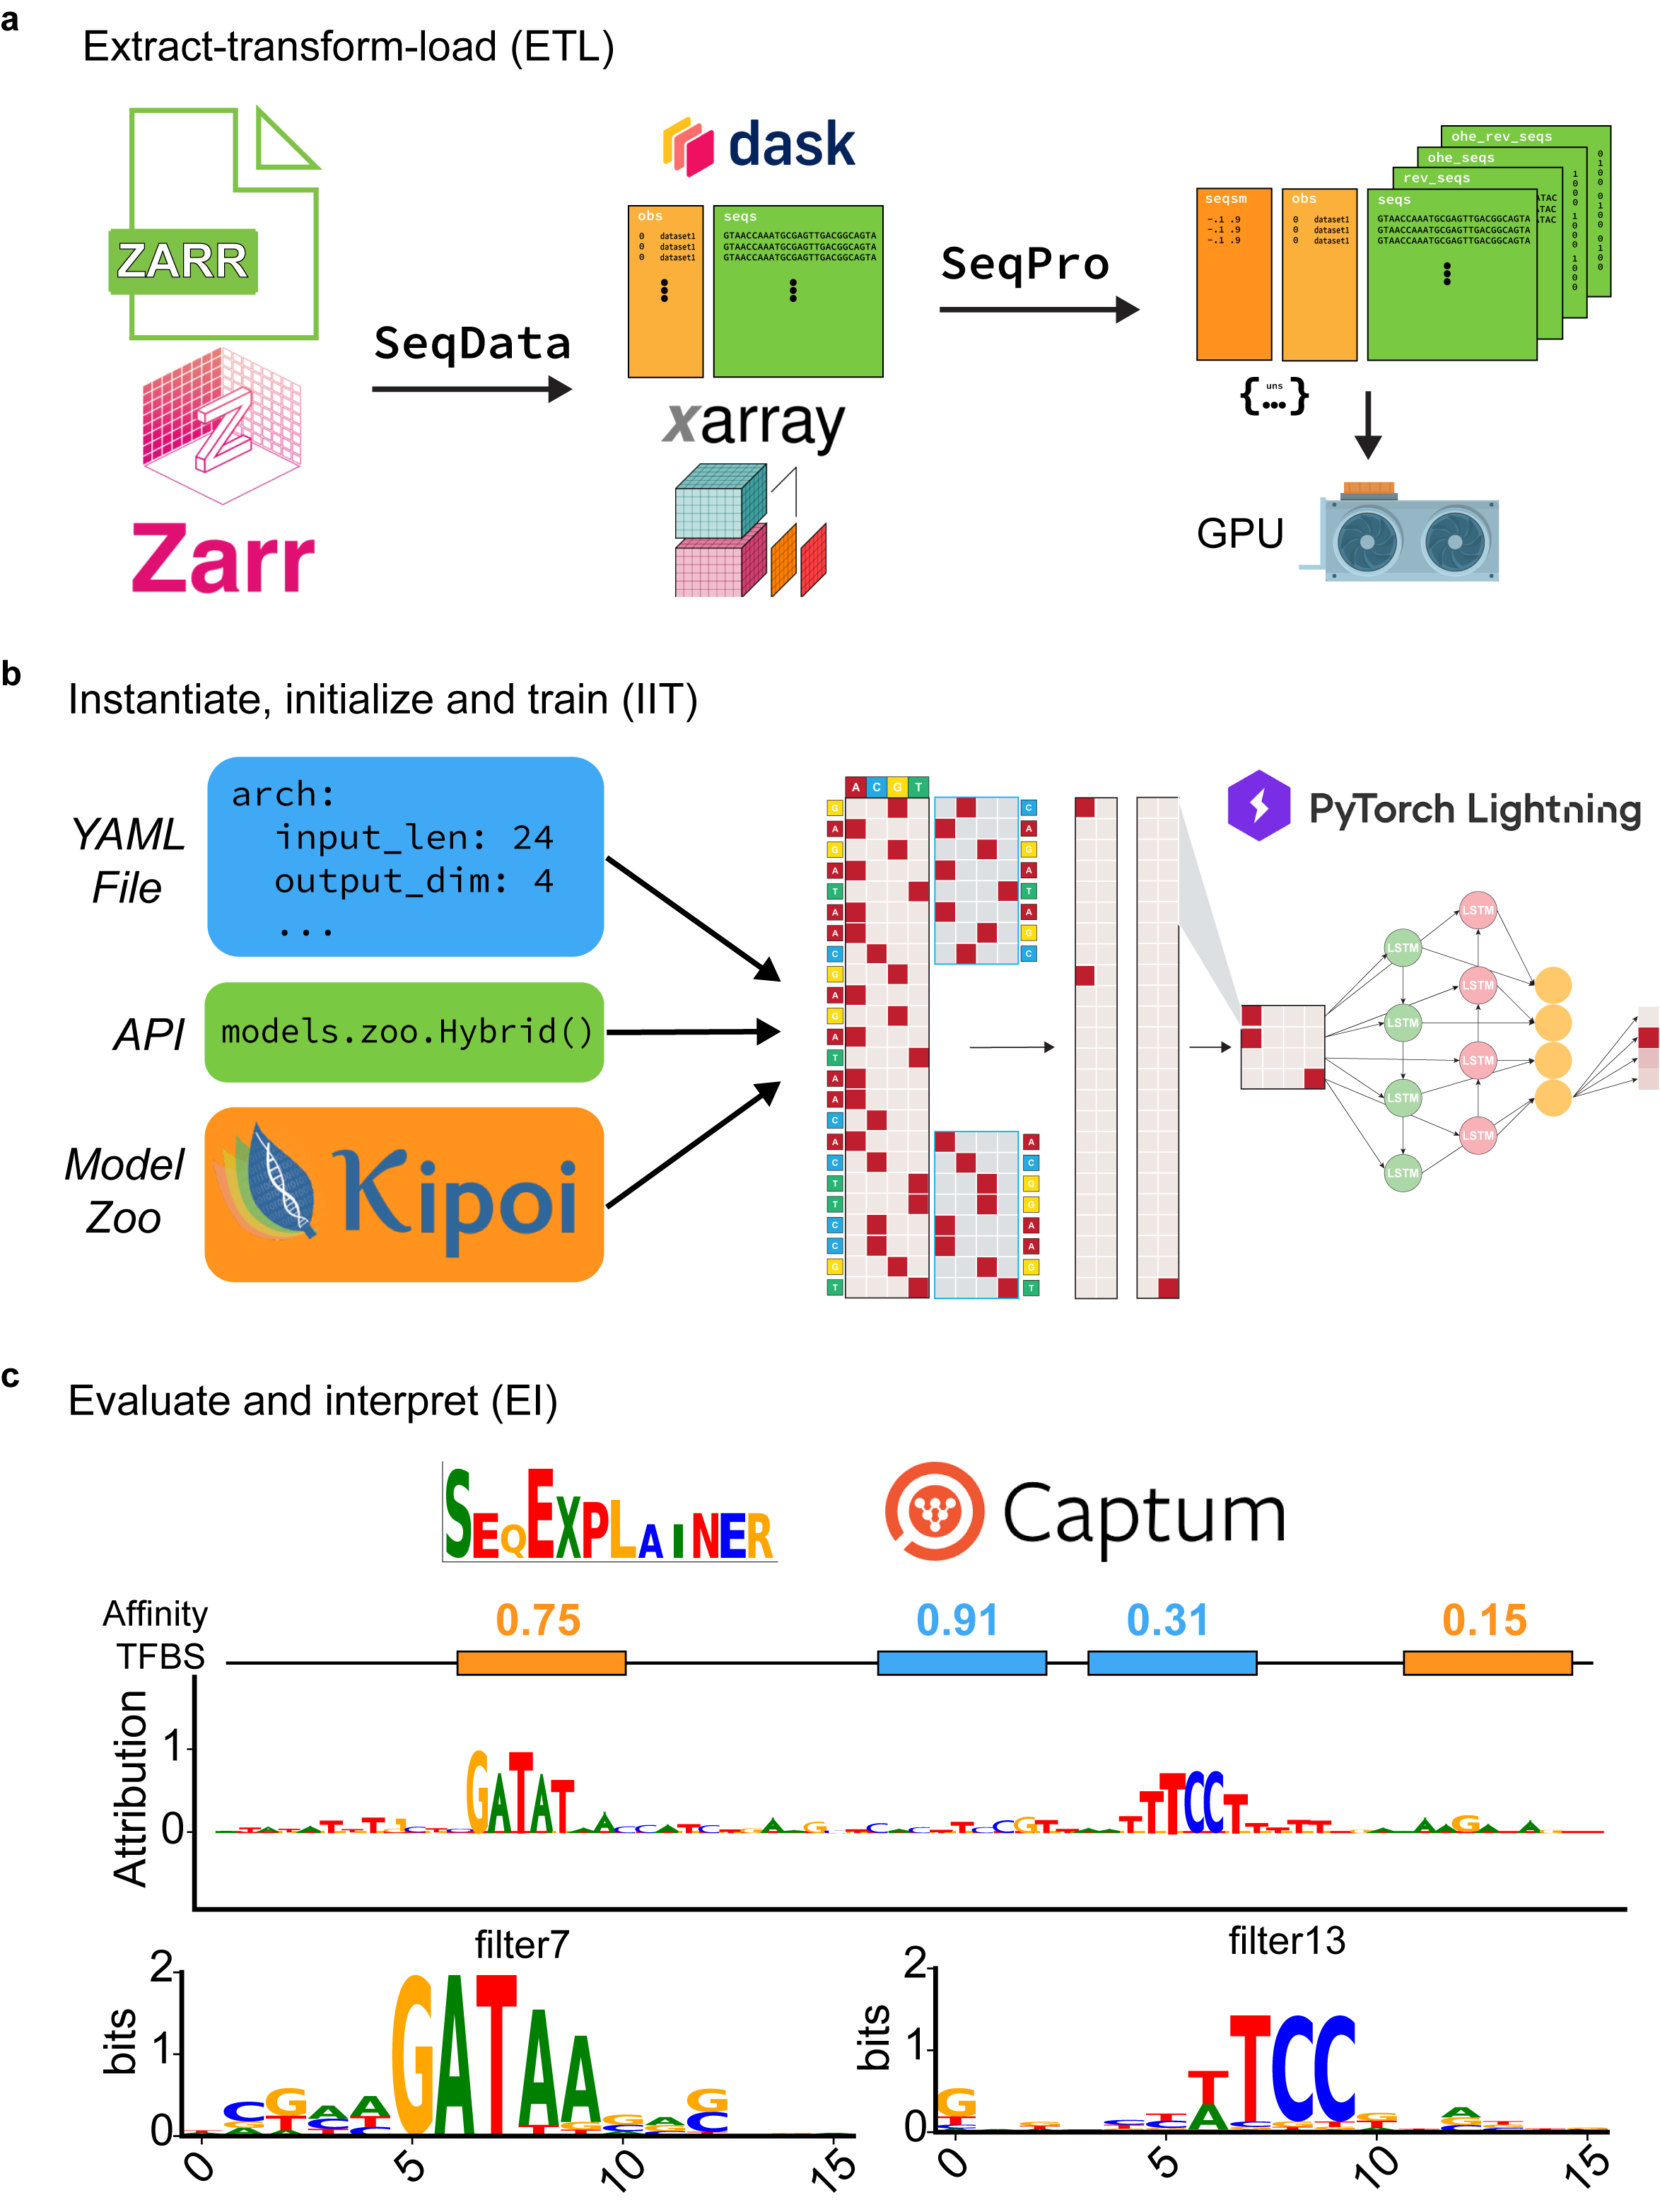
\includegraphics[width=0.9\textwidth, height=0.745\textheight]{1_figures-and-files/figure1.png}
    \caption[EUGENe workflow overview]{\textbf{EUGENe workflow for predictive analyses of regulatory sequences}. The EUGENe workflow can be broken up into three primary stages: \textbf{a}, data extraction, transformation and loading (ETL), \textbf{b}, model instantiation, initialization and training (IIT), and \textbf{c}, model evaluation and interpretation (EI). The ETL stage (\textbf{a}) begins with using the SeqData subpackage to create Dask enhanced, XArray datasets backed by Zarr stores. Data transformation is handled by the SeqPro subpackage, after which data can be loaded into graphical processing units (GPUs). In the subsequent IIT stage (\textbf{b}), model architectures (such as the example shown in the schematic) are instantiated from configuration files (in YAML format) from the EUGENe application programming interface (API) or from Kipoi. EUGENe then uses PyTorch Lightning for training these architectures. The subpackage SeqExplainer (which is backed by the Captum package) is used for model interpretation in the EI stage (\textbf{c}). Common visualizations produced by SeqExplainer include the logos depicted for an example input sequence (top) or for convolutional filters (bottom).}
    \label{fig:1 Figure 1}
\end{figure}

A standard EUGENe workflow consists of 3 main stages outlined in \textbf{Figure~\ref{fig:1 Figure 1}}: extracting, transforming and loading (collectively ETL) data from common file formats (\textbf{Figure~\ref{fig:1 Figure 1}a}), instantiating, initializing and training (collectively IIT) neural network architectures (\textbf{Figure~\ref{fig:1 Figure 1}b}), and evaluating and interpreting (EI) learned model behavior on held-out data (\textbf{Figure~\ref{fig:1 Figure 1}c}). The major goal of EUGENe is to streamline the end-to-end execution of these three stages to promote the effective design, implementation, validation and interpretation of DL solutions in regulatory genomics. We have listed several common DL for regulatory genomics tasks that can be implemented in an end-to-end fashion with EUGENe (\textbf{Supplementary Table 1}). We next describe three in detail, highlighting the core aspects of the workflow on different data types and training tasks. A more detailed description of the workflow is provided in the Methods section.

\begin{figure}[p]
    \centering
    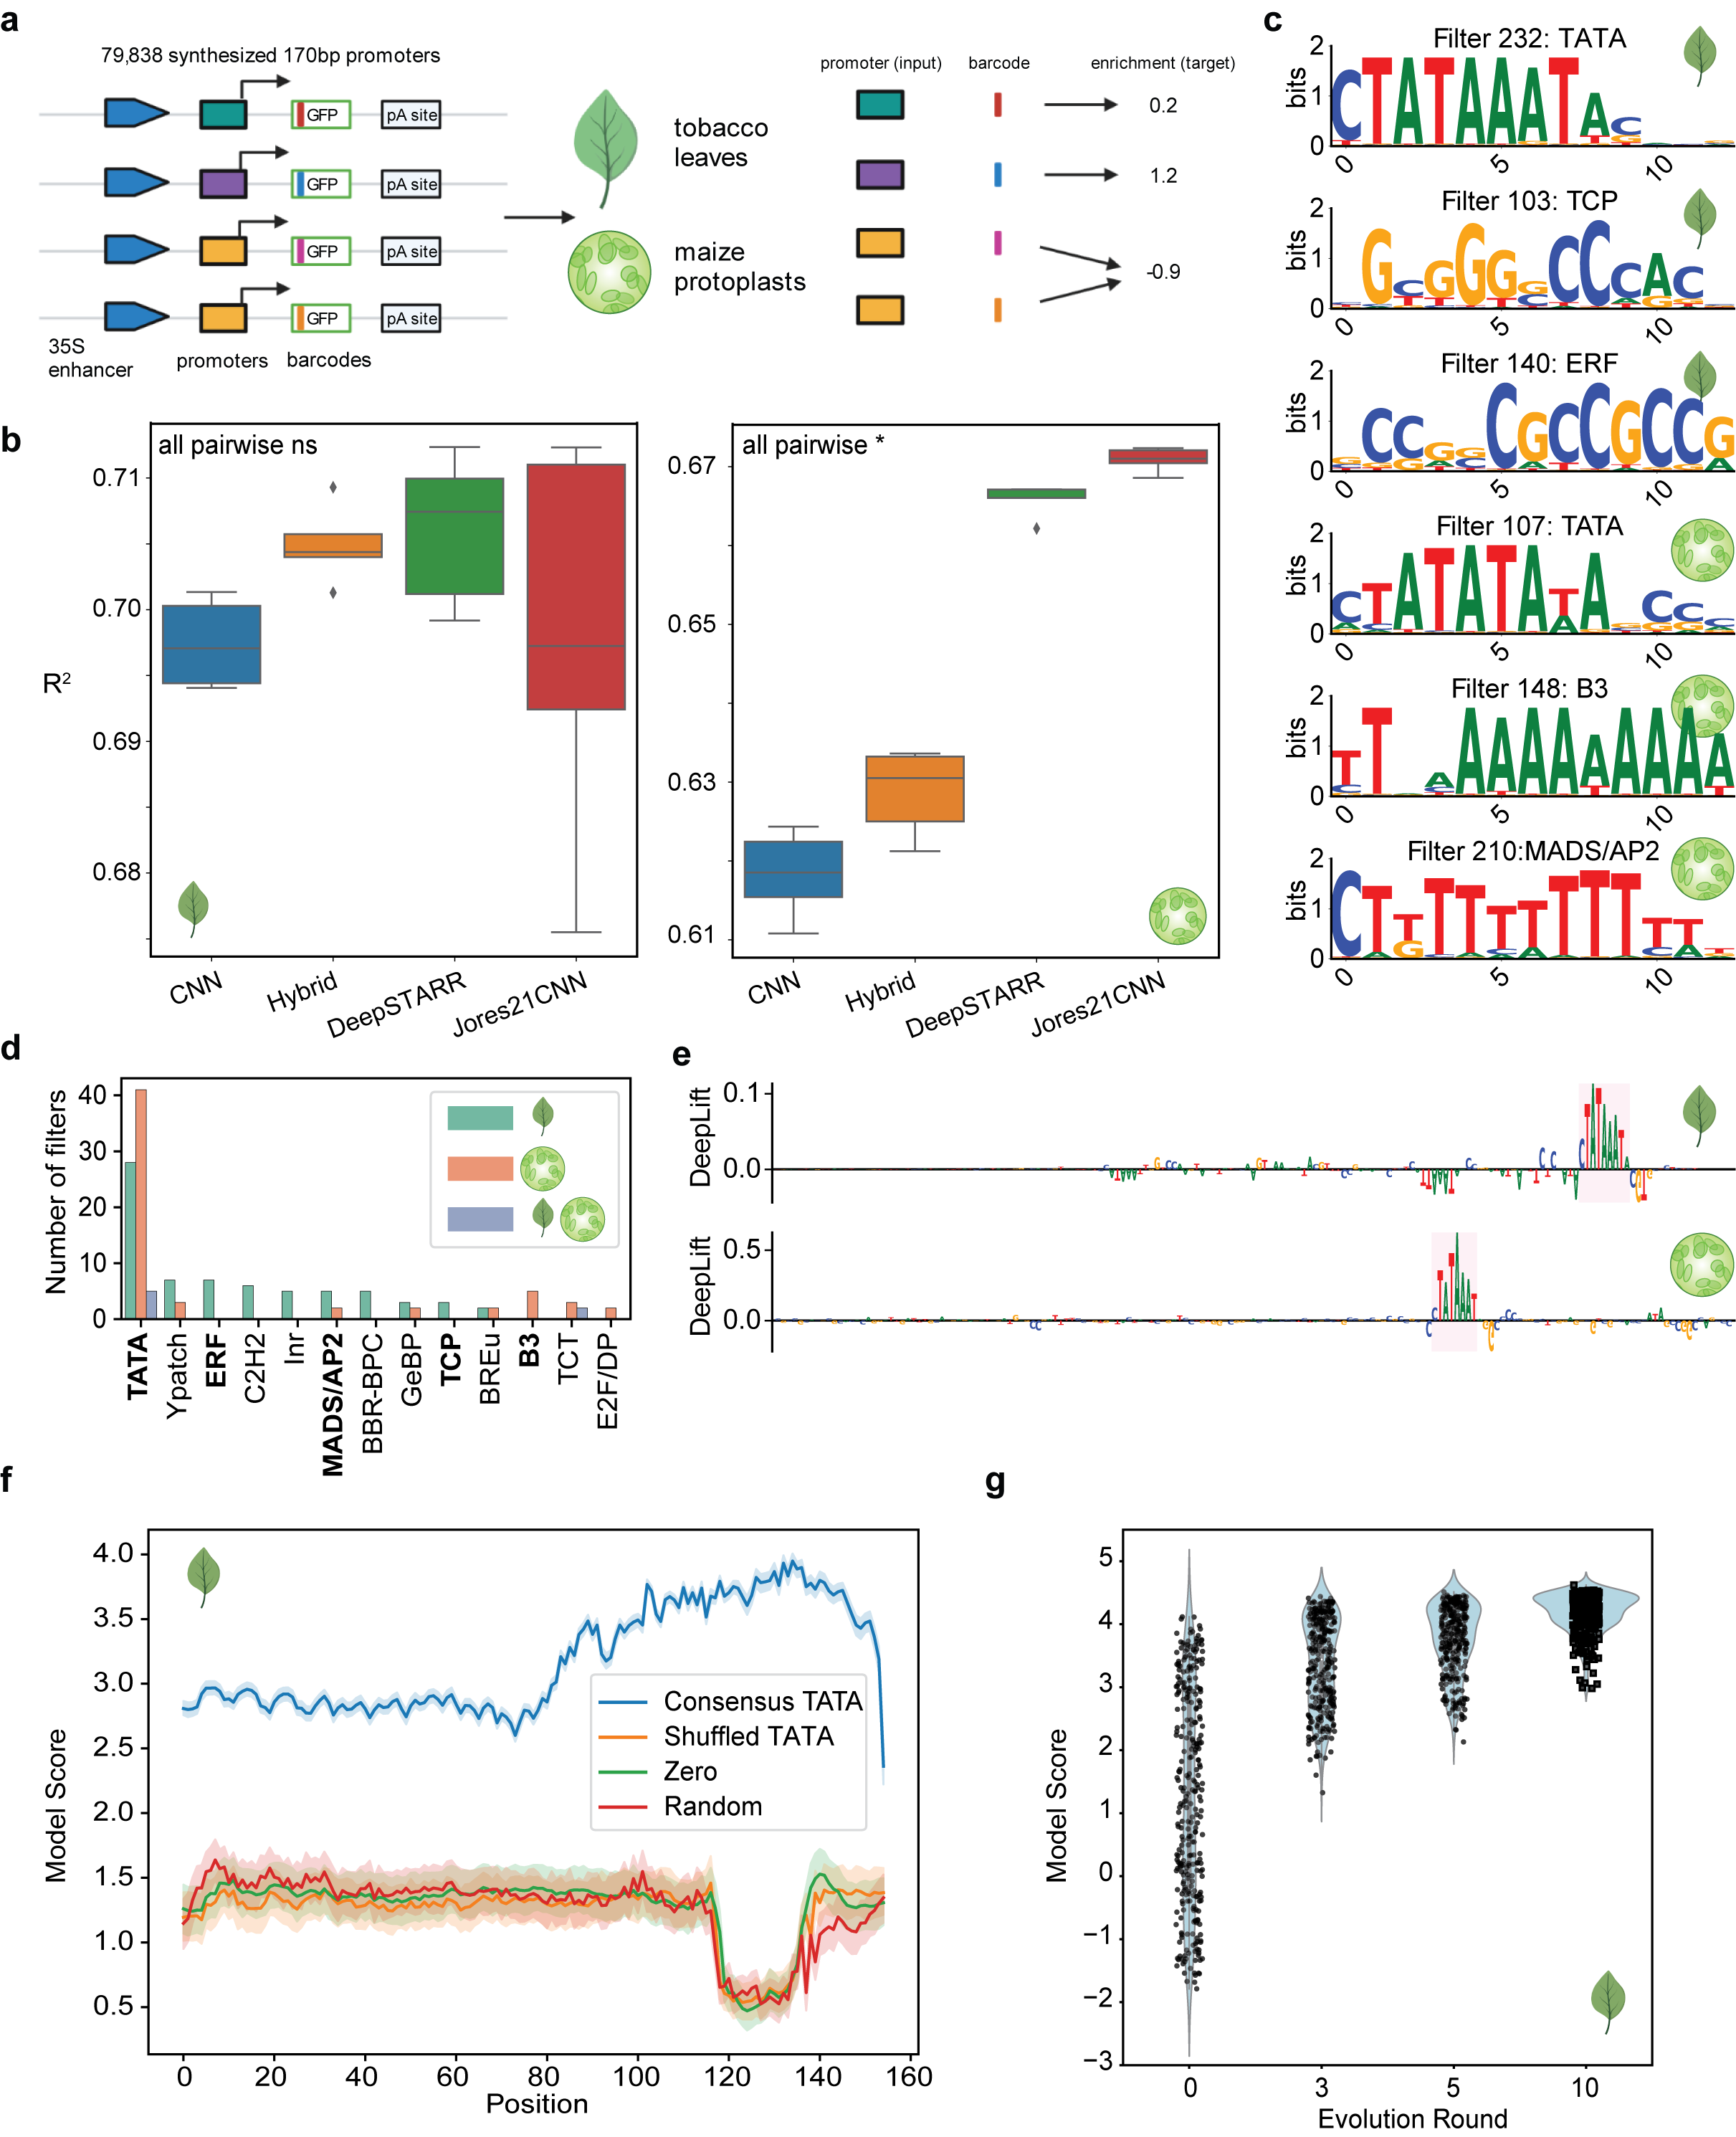
\includegraphics[width=0.9\textwidth, height=0.745\textheight]{1_figures-and-files/figure2.png}
    \caption[STARR-seq plant promoter activity prediction]{\textbf{STARR-seq plant promoter activity prediction}. \textbf{a}, jores21 use case schematic. We trained EUGENe models to predict the regulatory activity of 79,838 plant promoters quantified by plant STARR-seq in tobacco and maize. \textbf{b}, Performance comparison of four convolution-based architectures on predicting promoter activity in tobacco leaves (left) and maize protoplasts (right). The boxplots show distributions of R2 values on held-out test data for each architecture across n=5 independent experiments (random initializations). The boxes show medians along with low and high quartiles. Whiskers extend to the furthest datapoint within 1.5 times the interquartile range. More extreme points are marked as outliers. A two-sided Mann-Whitney U test was used to determine p-values which were adjusted by the Benjamini-Hochberg method (* = p < 0.05, ns = not significant). Test statistics and adjusted p-values for the leaf models (left) were: CNN-Hybrid (u=15, adjusted p-value=0.01), CNN-DeepSTARR (u=24, adjusted p-value=0.17), CNN-Jores21CNN (u=12, adjusted p-value=1.0), Hybrid-DeepSTARR (u=17, adjusted p-value=1.0), Hybrid-Jores21CNN (u=22, adjusted p-value=1.0), DeepSTARR-Jores21CNN (u=14, adjusted p-value=0.84). Test statistics and adjusted p-values for the protoplast models (right) were: CNN-Hybrid (u=15, adjusted p-value=0.03), CNN-DeepSTARR (u=24, adjusted p-value=0.01), CNN-Jores21CNN (u=12, adjusted p-value=0.01), Hybrid-DeepSTARR (u=17, adjusted p-value=0.01), Hybrid-Jores21CNN (u=22, adjusted p-value=0.01), DeepSTARR-Jores21CNN (u=14, adjusted p-value=0.01). \textbf{c}, A hand selected set of convolutional filters visualized as PWM logos that had significant annotations to known core promoter elements (CPE) and transcription factor (TF) binding clusters in plants. \textbf{d}, Histogram showing the number of learned filters assigned to CPEs and TF binding clusters by TomTom with bolded annotations corresponding to the logos in \textbf{c}. \textbf{e}, Sequence logo visualizations of feature importance scores calculated using the DeepLIFT algorithm on the highest predicted test set sequence in the Hybrid leaf (top) and Jores21CNN protoplast (bottom) model. \textbf{f}, Model scores for n=310 sequences implanted with a 16bp sequence containing a consensus TATA box motif, a shuffled version of the same sequence, an all zeros sequence and a random sequence (all 16bp in length). Mean model scores with 95\% confidence intervals are shown. \textbf{g}, Model scores for the same set of n=310 promoters at different rounds of evolution compared against baseline predictions (evolution round 0). The best Hybrid leaf model was used to generate panels \textbf{c}, \textbf{d}, \textbf{f} and \textbf{g} (protoplast model results are shown in Supplementary Figure 1). Source data are provided in the Figure2\_SourceData.zip file.}
    \label{fig:2 Figure 2}
\end{figure}

We first used EUGENe to analyze published data from an assay of plant promoters\cite{Jores2021-iu} (\textbf{Figure~\ref{fig:2 Figure 2}a}). Jores et al selected promoter sequences from -165 to +5-bp relative to the annotated transcription start site (TSS) for protein-coding and microRNA (miRNA) genes of \textit{Arabidopsis thaliana}, \textit{Zea mays} (maize), and \textit{Sorghum bicolor}. A total of 79,838 170-bp promoters were used to transiently transform two separate plant systems, tobacco leaves and maize protoplasts. Regulatory activity was quantified using a variant of the self-transcribing active regulatory region sequencing (STARR-seq) assay\cite{Jores2020-hm} in each system. The resulting data provides two activity scores that can serve as single task regression targets for training EUGENe models.

We implemented both the custom BiConv1D layer\cite{Onimaru2020-do} and CNN architecture (Jores21CNN) described in Jores et al, and then trained separate Jores21CNN architectures for predicting tobacco leaf (leaf models) and maize protoplast (protoplast models) activity scores. We benchmarked these models against built-in CNN and Hybrid architectures with matched hyperparameters, as well as a DeepSTARR architecture\cite{De_Almeida2022-aa} (Supplementary Data 1). As described in Jores et al (see Methods), we initialized 78 filters of the first convolutional layer of all models with position weight matrices (PWMs) of plant transcription factors (n=72) and core promoter elements (n=6)\cite{Jores2021-iu}. In both systems, performance metrics for the most predictive models were comparable to those reported in Jores et al (\textbf{Figure~\ref{fig:2 Figure 2}b}, \textbf{Supplementary Figure~\ref{fig:supplementary_1}a}). We also trained models on activity scores from both leaves and protoplasts (combined models) and noted a marked drop in performance (\textbf{Supplementary Figure~\ref{fig:supplementary_1}b}), underscoring differences in the way the leaf and maize systems interact with the same set of promoters\cite{Jores2021-iu}.

We next applied several of EUGENe’s interpretation functions to the trained models to determine the sequence features each used to predict plant promoter activity. First, we used a filter visualization approach\cite{Minnoye2020-vz} to generate position frequency matrix (PFM) representations for each of the first convolutional layer’s filters and applied the TomTom\cite{Gupta2007-zw} tool to annotate them. We queried the PFMs against the 78 motifs used to initialize the convolutional layers, both to determine if the initialized filters retained their motifs and to see if randomly initialized filters learned them de novo. For the leaf and protoplast models, many of the learned filters were annotated to the TATA box binding motif and other core promoter elements (\textbf{Figure~\ref{fig:2 Figure 2}c}\textbf{d}). Only 10 learned filters from the combined model were assigned a significant annotation by TomTom (\textbf{Figure~\ref{fig:2 Figure 2}d}, \textbf{Supplementary Figure~\ref{fig:supplementary_1}c}), consistent with the observed performance drop in this system (\textbf{Supplementary Figure~\ref{fig:supplementary_1}a}). Next, we applied the DeepLIFT method\cite{Shrikumar2016-lf} to determine the individual nucleotide contributions for each test set sequence prediction. For many of the sequences with the highest observed activity scores, the TATA box motifs were often the lone salient feature identified (\textbf{Figure~\ref{fig:2 Figure 2}e}, \textbf{Supplementary Figure~\ref{fig:supplementary_1}d}). In fact, when only a TATA box motif was inserted into every possible position in each of 310 selected promoters, we observed a 147\% average increase in predicted activity across insertion positions and sequence contexts for the leaf model (\textbf{Figure~\ref{fig:2 Figure 2}f}, \textbf{Supplementary Figure~\ref{fig:supplementary_1}e}). Finally, we performed 10 rounds of in silico evolution on the same set of 310 promoters as described in Jores et al. Almost all starting promoters showed a significant increase in predicted activity after just three mutations (\textbf{Figure~\ref{fig:2 Figure 2}g}, \textbf{Supplementary Figure~\ref{fig:supplementary_1}f}). These results showcase a representative example of the way EUGENe’s interpretation suite can be used to identify the key features that a model uses to make predictions.

\begin{figure}[p]
    \centering
    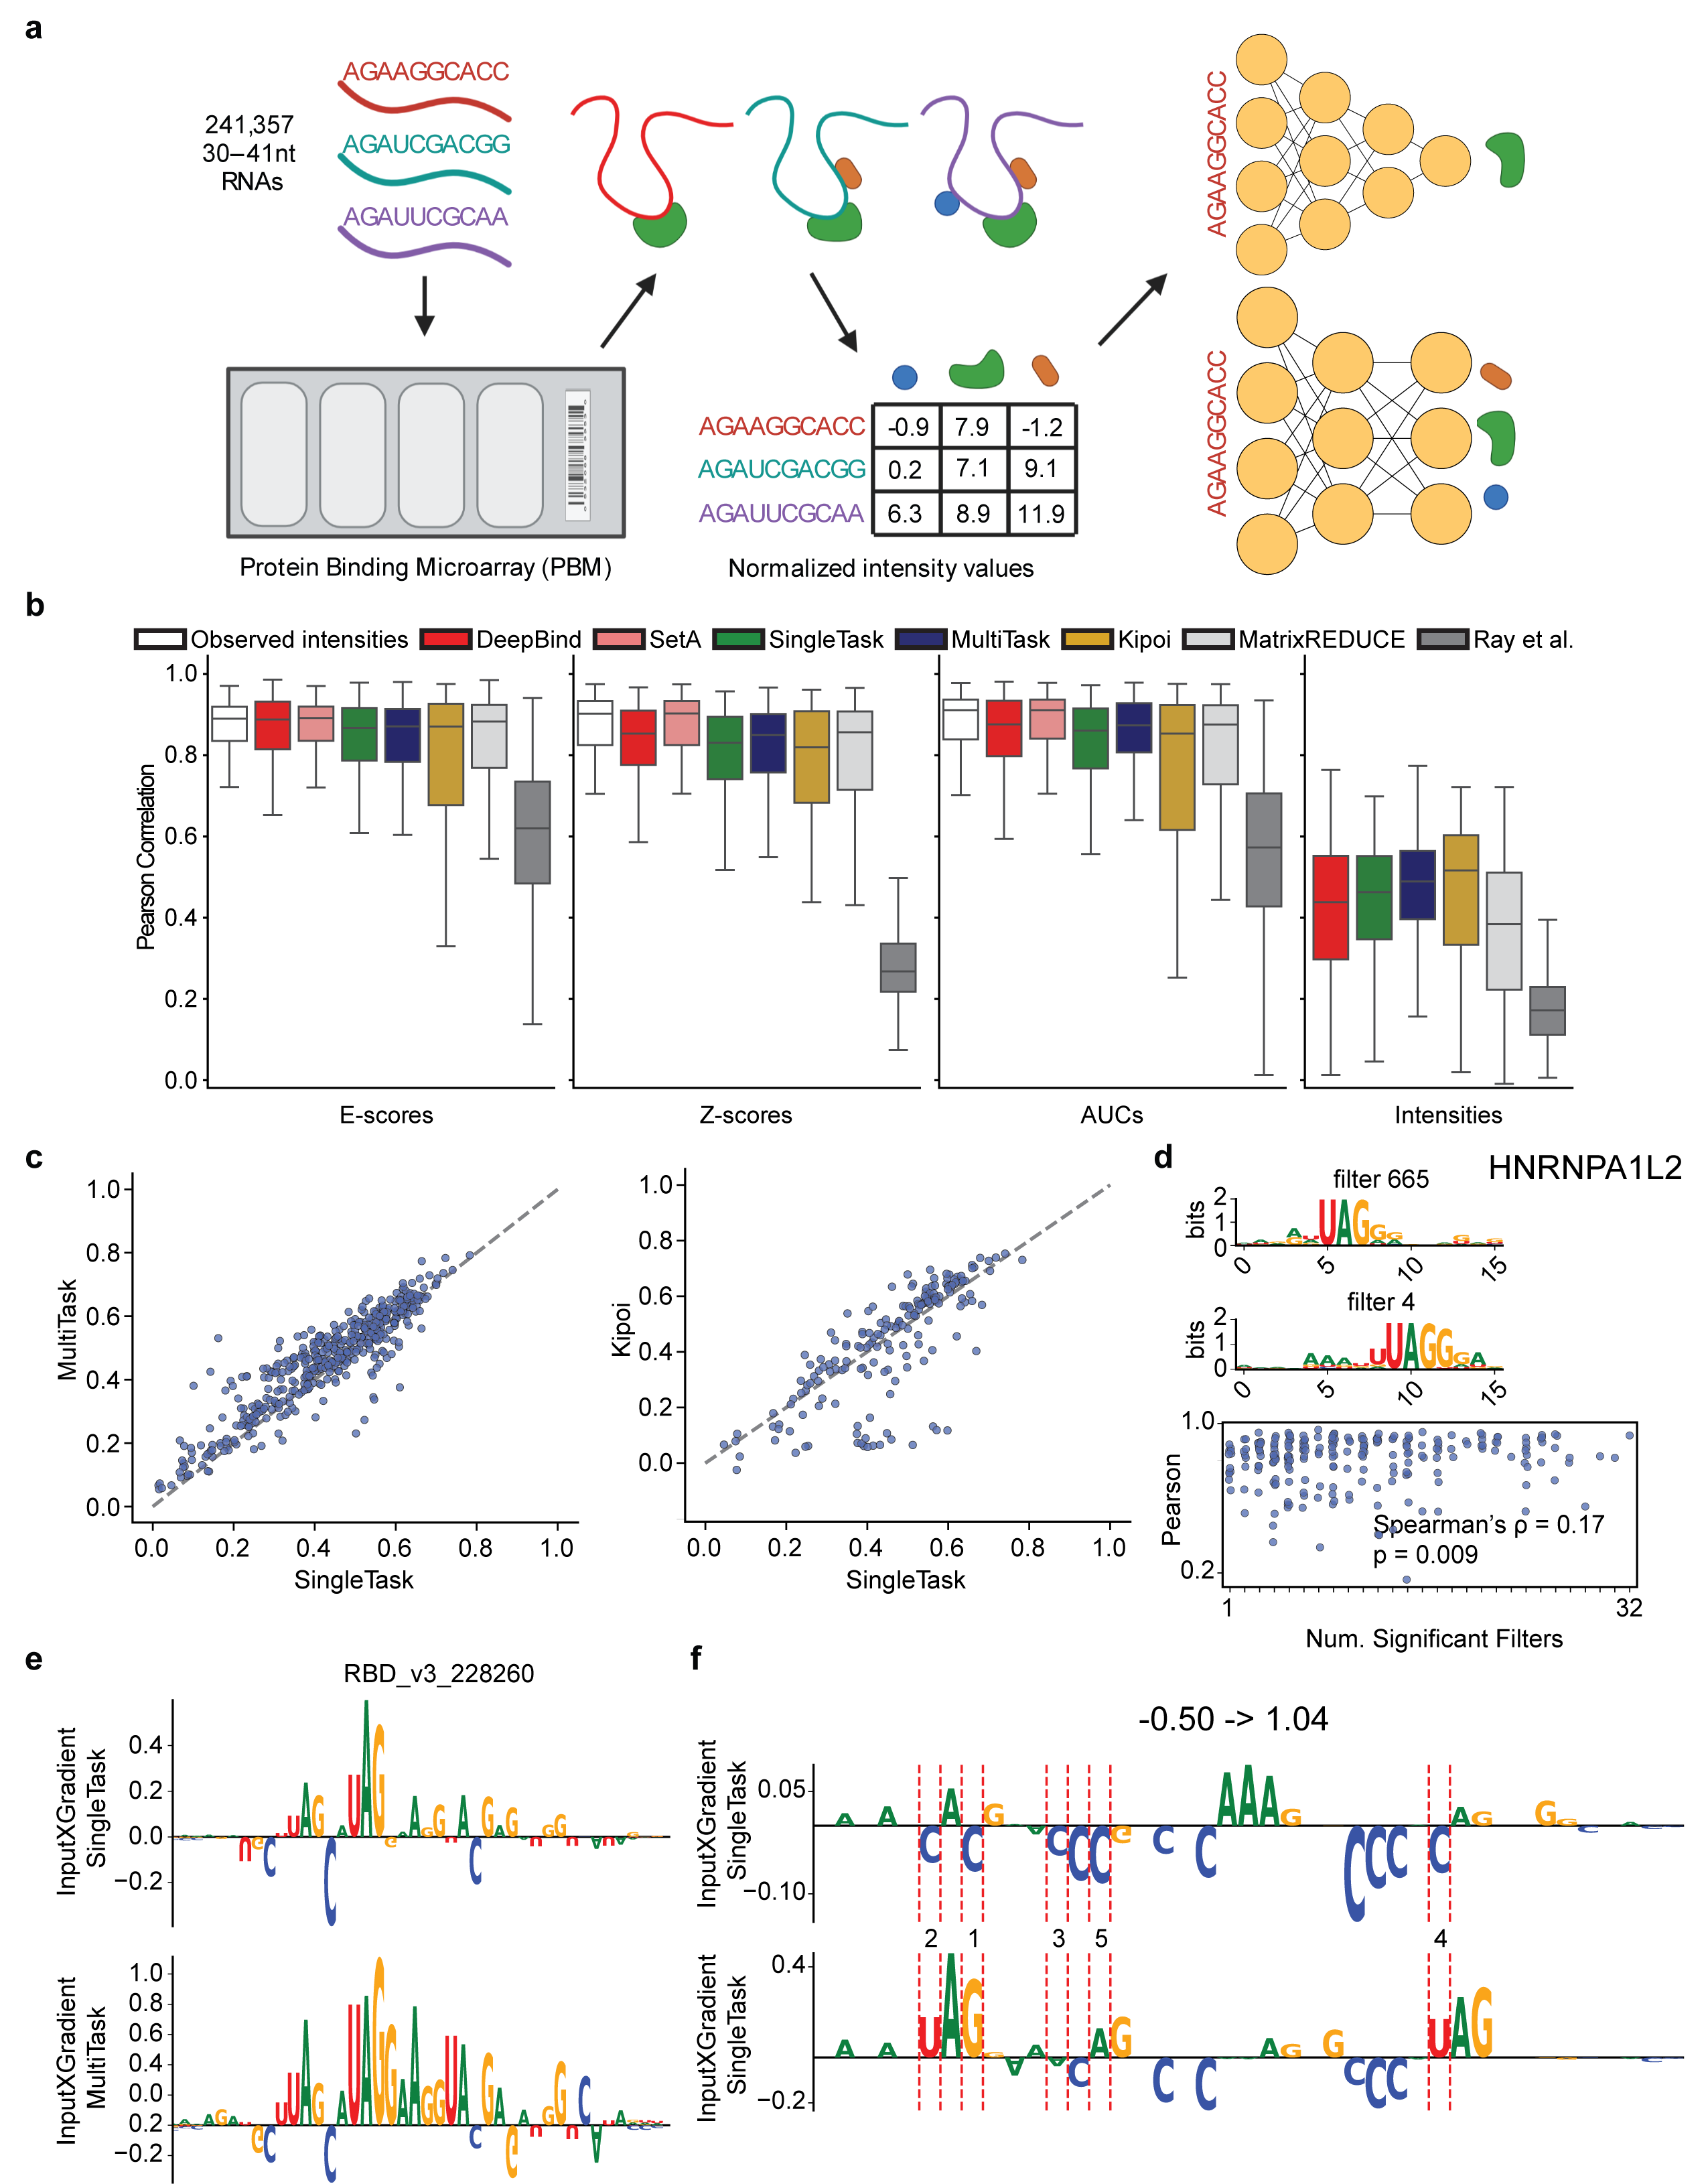
\includegraphics[width=0.9\textwidth, height=0.745\textheight]{1_figures-and-files/extended_data_figure1.png}
    \caption[In vitro RNA binding prediction with DeepBind]{\textbf{In vitro RNA binding prediction with DeepBind}. \textbf{a}, ray13 use case schematic. n=244 RNA binding proteins (RBPs) were assayed across a set of 241,357 RNA probes to generate a 241,357 x 244 dimensional matrix of normalized intensity values. \textbf{b}, Pearson correlations across four different metrics with each metric calculated from comparisons between observed (Set B) and predicted binding intensities (see Methods for more details on how each metric is calculated). Each boxplot indicates a distribution of Pearson correlations across all n=244 RBPs, except for Kipoi which includes n=89 RBPs. Ray et al, MatrixREDUCE, DeepBind and Observed intensities refer to correlations calculated from predicted intensities reported in Alipanahi et al. Observed intensities and SetA refer to correlations calculated using the intensities from Set A probes as the predicted intensities (see Methods). The boxes show medians along with low and high quartiles. Whiskers extend to the furthest datapoint within 1.5 times the interquartile range. \textbf{c}, Performance comparison scatterplots for ST models against MT models (left) and against Kipoi models (right). Each dot indicates a comparison of the Pearson correlation between predicted and observed intensities for two models on a single RBP. \textbf{d}, (top) A multitask filter with a TomTom significant annotation for HNRNPA1L2 visualized as a PWM logo. (middle) A filter for the single task HNRNPA1L2 model with a significant TomTom annotation for HNRNPA1L2. (bottom) The relationship between multitask performance (using the Z-scored Pearson correlations of observed and predicted intensities) on the y-axis, against the number of filters that were annotated with the corresponding RBP for that task on the x-axis. The Spearman’s correlation coefficient and associated p-value are shown. \textbf{e}, Attributions for the sequence with the highest observed intensity in the test set for HNRNPA1L2. The attributions were calculated using InputXGradient for single task (top) and multitask (bottom) models. \textbf{f}, The InputXGradient attribution scores for a random (top) and evolved (bottom) sequence after evolution with the HNRNPA1L2 single task model. Red dashed lines indicate mutations made during evolution and are annotated with the round the mutation occurred in. Source data are provided in the ExtendedFigure1\_SourceData.zip file.}
    \label{fig:3 Figure 3}
\end{figure}

To illustrate EUGENe’s versatility for different inputs and prediction tasks, we next applied it to analyze RNA binding protein (RBP) specificity data introduced in Ray et al\cite{Ray2013-yd} and analyzed with DL in Alipanahi et al\cite{Alipanahi2015-ef}. In the latter work, they trained 244 CNN models (DeepBind models) that each predicted the binding patterns of a single RBP on a set of 241,357 RNA probes (\textbf{Figure~\ref{fig:3 Figure 3}a}). The full probe set was designed to capture all possible RNA 9-mers at least 16 times and was split into two balanced subsets, Set A and Set B, for training and validation respectively (see Methods)\cite{Ray2013-yd}. Each RBP was incubated with a molecular excess of probes from each subset (in separate experiments) and subsequently recovered by affinity purification. The RNAs associated with each RBP were then quantified by microarray and subsequent bioinformatic analysis\cite{Berger2009-la}. This yielded a vector of continuous binding intensity values for each RBP across the probe set that can be used for prediction.

To prepare for training, we first implemented a flexible DeepBind architecture in EUGENe (see Methods), and then trained 244 single task models using a nearly identical training procedure to Alipanahi et al. (Supplementary Data 2). Along with these single task models, we also randomly initialized and trained a multitask model (Supplementary Data 2) to predict 233 RBP specificities (i.e. a 233 dimensional vector) in a single forward pass, excluding 11 RBPs due to a high proportion of missing values across probes in the training set. We also loaded 89 existing Kipoi\cite{Avsec2019-ke} models trained on a subset of human RBPs in the dataset.

Performance on Set B for all deep learning models was on par with Set B’s correlation to Set A (\textbf{Figure~\ref{fig:3 Figure 3}b}, \textbf{Supplementary Figure~\ref{fig:supplementary_2}a}) and both single task and multitask models trained with EUGENe showed comparable performance to Kipoi and DeepBind models (\textbf{Figure~\ref{fig:3 Figure 3}b}\textbf{c}, \textbf{Supplementary Figure~\ref{fig:supplementary_2}a}\textbf{b}). The reason for the poor observed performance of certain Kipoi models is not immediately clear, but could relate to differences in sequence or target preprocessing prior to evaluation. Though the ability to load these pretrained models from Kipoi is very useful for benchmarking, implementing and retraining models is often necessary for fair comparisons of performance. EUGENe supports both loading and retraining models, allowing users to more quickly design and execute quality benchmarking experiments. 

We next applied EUGENe’s interpretation suite to our trained models, first using the filter visualization approach outlined in Alipanahi et al to generate PFMs for convolutional filters. We again used TomTom to identify filters annotated with canonical RBP motifs\cite{Ray2013-yd} in both the best performing single task models and the multitask model (\textbf{Figure~\ref{fig:3 Figure 3}d}, \textbf{Supplementary Figure~\ref{fig:supplementary_2}c}) and found that the number of multitask filters annotated to an RBP was correlated with predictive performance for that RBP (\textbf{Figure~\ref{fig:3 Figure 3}d}, bottom). We also calculated attributions for all Set B sequences using the InputXGradient method\cite{Shrikumar2016-lf} and observed that canonical motifs were learned by both single task and multitask models (\textbf{Figure~\ref{fig:3 Figure 3}e}, \textbf{Supplementary Figure~\ref{fig:supplementary_2}d}). Finally, we used EUGENe’s sequence evolution functionality to evolve 10 random sequences using the single task HNRNPA1L2 model and visualized the attributions for these sequences before and after five rounds of evolution (\textbf{Figure~\ref{fig:3 Figure 3}f}). Several of the mutations that most increased the predicted score were those that generated canonical binding motifs for the protein. We repeated this for two other RBPs (Pcbp2 and NCU02404) and observed that each model prioritizes mutations that create canonical binding motifs specific to the RBP they were trained on (\textbf{Supplementary Figure~\ref{fig:supplementary_2}e}). These results show that EUGENe simplifies the extraction of salient features from models trained within the same workflow.

\begin{figure}[p]
    \centering
    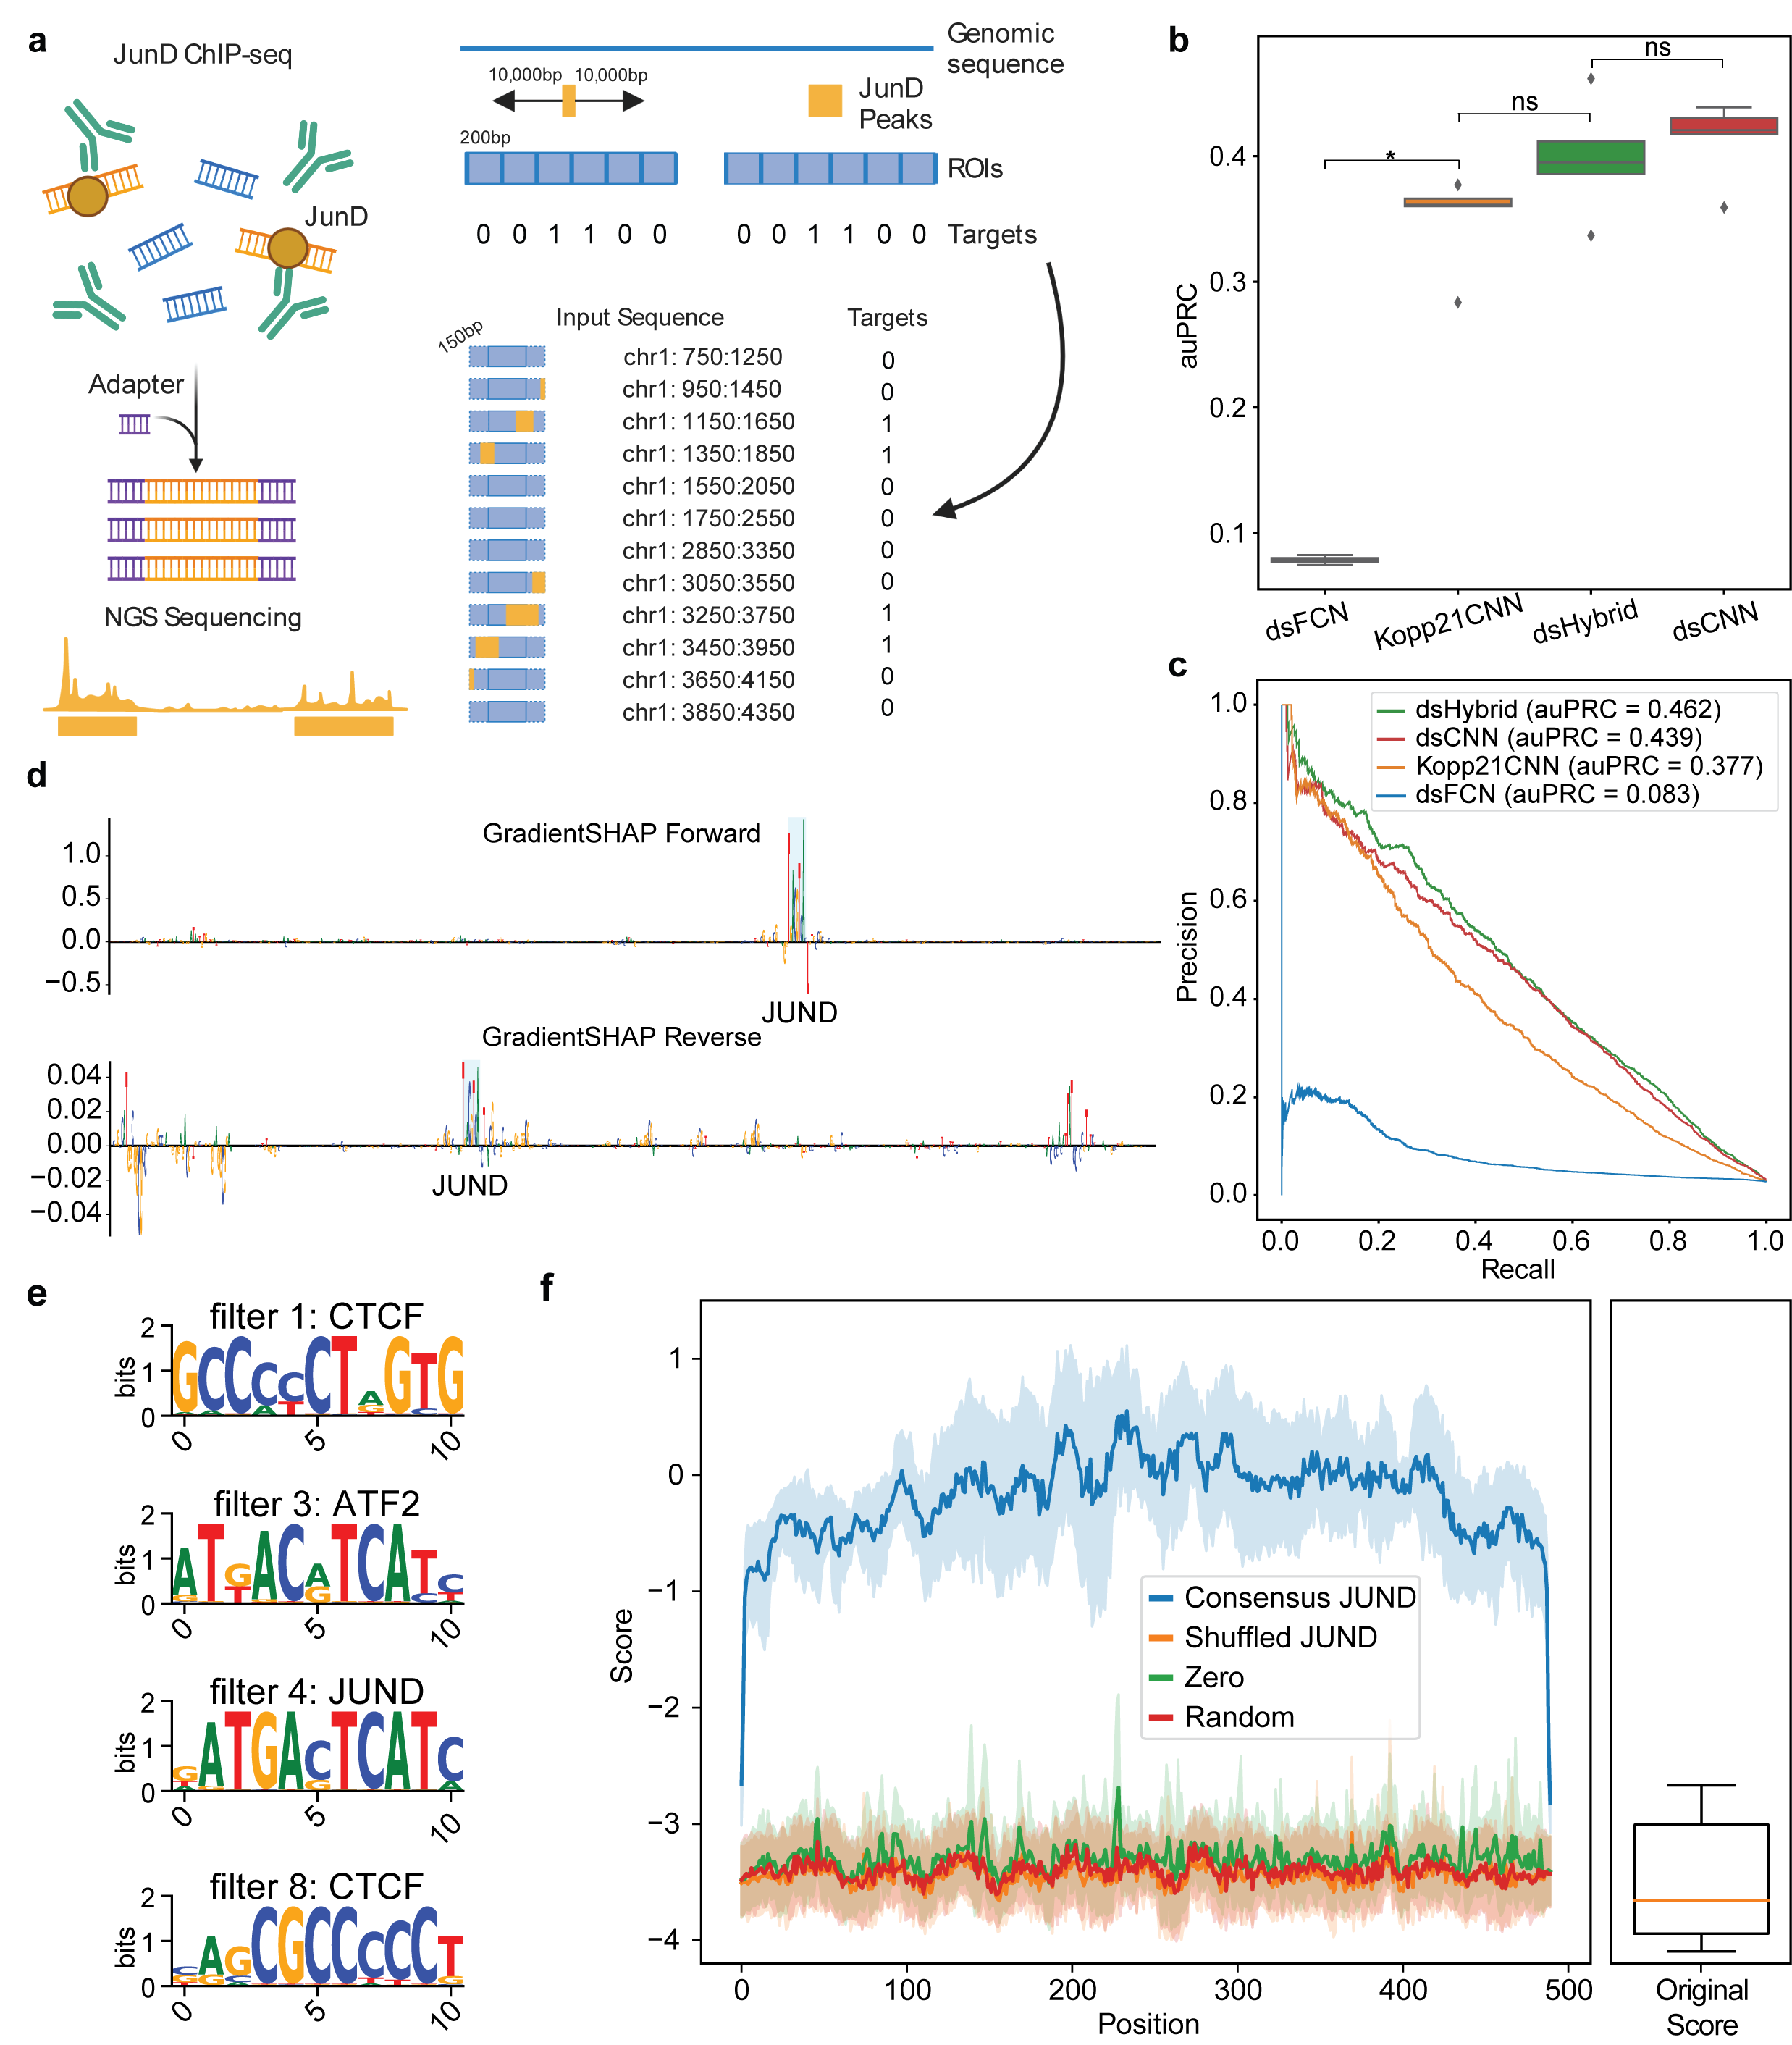
\includegraphics[width=0.9\textwidth, height=0.745\textheight]{1_figures-and-files/extended_data_figure2.png}
    \caption[JunD ChIP-seq binding classification]{\textbf{JunD ChIP-seq binding classification}. \textbf{a}, kopp21 use case schematic. We used SeqData to load in a set of 11,086 ChIP-seq peaks for JunD and to generate positive and negative sets for JunD binding prediction. SeqData uses a set of regions of interest (ROIs) along with peaks and a bin size and outputs a set of labeled sequences for each bin in the ROI. Bins are labeled as positive (1) if they overlap a peak and negative (0) if they do not. Upon loading, each sequence is extended by 150bp in each direction to provide more sequence context for prediction. \textbf{b}, \textbf{c}, auPRCs on held-out test data from chromosome 3 for JunD binding classification across four double-stranded architectures \textbf{b}, The boxplots show distributions of auPRC values on held-out test data for each architecture across n=5 independent experiments (random initializations). A two-sided Mann-Whitney U test was used to determine p-values which were adjusted by the Benjamini-Hochberg method  (* = p < 0.05, ns = not significant). Test statistics and adjusted p-values were: dsFCN-Kopp21CNN (u=0, adjusted p-value=0.02), dsFCN-dsHybrid (u=0, adjusted p-value=0.02), dsFCN-dsCNN (u=0, adjusted p-value=0.02), Kopp21CNN-dsHybrid (u=4, adjusted p-value=0.11), Kopp21CNN-dsCNN (u=4, adjusted p-value=0.11), dsHybrid-dsCNN (u=8, adjusted p-value=0.42). \textbf{c}, auPR curves for the best models from each architecture. \textbf{d}, Sequence logos of attributions for the top predicted sequence. The top row shows attributions from the forward strand and the bottom row from the reverse strand. Attributions were calculated using GradientSHAP. \textbf{e}, A selected set of convolutional filters visualized as PWM logos with significant annotations from TomTom. \textbf{f}, Model scores for n=10 random sequences with consensus JunD motif implanted at each possible location. Mean model scores with 95\% confidence intervals are shown. The boxplot shows the distribution of scores for the random sequences prior to JunD motif implantation. All boxes show medians along with low and high quartiles. Whiskers extend to the furthest datapoint within 1.5 times the interquartile range. More extreme points are marked as outliers. Source data are provided in the ExtendedFigure2\_SourceData.zip file.}
    \label{fig:4 Figure 4}
\end{figure}

As our final use case, we applied EUGENe to the classification of JunD binding as described in Kopp et al\cite{Kopp2020-fw}. This task utilizes ChIP-seq data from ENCODE\cite{ENCODE_Project_Consortium2012-tn} to generate input sequences and binarized classification labels for each sequence (\textbf{Figure~\ref{fig:4 Figure 4}a}). We used EUGENe to first build a DL-ready dataset for this prediction task (see Methods), then implemented the CNN architecture described in Kopp et al (Kopp21CNN). We benchmarked classification performance against built-in FCNs, CNNs, and Hybrid models with matched hyperparameters (Supplementary Data 3). All built-in models were configured to incorporate information from both the forward and reverse strand (double stranded or “ds” models). 

We trained models using the same procedure described in Kopp et al (see Methods)\cite{Kopp2020-fw}. Due to the unbalanced nature of the dataset, we focused on evaluating models with the area under the precision recall curve (auPRC). For our Kopp21CNNs, we were able to achieve comparable performances on held out chromosome 3 sequences to those reported by Kopp et al for one-hot encoded sequences (\textbf{Figure~\ref{fig:4 Figure 4}b}\textbf{c}). The dsFCN, the only model without any convolutional layers, immediately overfit the data after a single training epoch and was not predictive of binding (\textbf{Figure~\ref{fig:4 Figure 4}c}). The dsCNN models, however, achieved higher mean auPRCs than dsHybrid models, and significantly higher auPRCs than Kopp21CNN architectures.

We next applied EUGENe’s interpretation tools to ask whether our best models were learning sequence features relevant to JunD binding to make predictions. We first generated attributions for the forward and reverse complement strands of all test set sequences using the GradientSHAP\cite{Lundberg2017-hh} method and visualized the most highly predicted sequences as sequence logos (\textbf{Figure~\ref{fig:4 Figure 4}d}, \textbf{Supplementary Figure~\ref{fig:supplementary_3}a}). We observed that the most important nucleotides often highlighted consensus or near consensus JunD motifs and that these motifs were often attributed similarly on both the forward and reverse strands (\textbf{Figure~\ref{fig:4 Figure 4}d}, \textbf{Supplementary Figure~\ref{fig:supplementary_3}a}). However, there were instances where salient motifs were highlighted on one strand but not the other (\textbf{Figure~\ref{fig:4 Figure 4}d}), indicating the utility of incorporating information from both strands for prediction. We next generated PFM representations for all 10 filters of each convolutional model (excluding dsFCNs) and annotated them using TomTom against the HOCOMOCO FULL v11 database\cite{Kulakovskiy2018-oz} (\textbf{Figure~\ref{fig:4 Figure 4}e}, \textbf{Supplementary Figure~\ref{fig:supplementary_3}b}). Among the top hits, we found several filters annotated with motifs such as JunD and CTCF (\textbf{Figure~\ref{fig:4 Figure 4}e}, \textbf{Supplementary Figure~\ref{fig:supplementary_3}b}). Finally, we performed an in silico experiment with the best overall model where we slid a consensus JunD motif across each position of a set of 10 randomly generated sequences and predicted binding (\textbf{Figure~\ref{fig:4 Figure 4}f}). We observed that the simple inclusion of the consensus binding site led to a significant jump in predicted output with some position specificity. These results once again showcase that EUGENe’s interpretation methods can help explain model predictions, in this case for DNA protein binding from a genome wide assay.

There are numerous opportunities for future development of EUGENe, but we see a few as high priority. EUGENe is primarily designed to work on nucleotide sequence input (DNA and RNA), but currently does not have dedicated functions for handling protein sequence or multi-modal inputs. Furthermore, as assays move from bulk to single cell resolution, it will be important to develop functionality for handling single cell data that allows users to easily ask questions about cell type specific regulatory syntax. Finally, we plan on expanding EUGENe’s dataset and model library to encompass a larger portion of those available in the field.

The heterogeneity in data types and methods that exist in DL for regulatory genomics and the rapid pace with which the field advances makes maintaining FAIR software in this space a major challenge. One of the tasks in \textbf{Supplementary Table 1}, for instance, involves a recently developed and highly specific data formatting and preprocessing pipeline\cite{Bravo_Gonzalez-Blas2019-fq}. The use of bespoke methods for data preprocessing, as well as for model interpretation, is quite common in the field, and is often necessary to train accurate models that avoid common machine learning pitfalls\cite{Whalen2021-fh}. For example, some workflows may require complex implementations of train and test set splitting to protect against information leakage\cite{Urban2020-ij}. We see substantial value in continuing to extend EUGENe into spaces such as these, and have designed the toolkit to allow for easy integration of this type of functionality. To continue to make bespoke methods and workflows accessible, we intend to encourage community development of EUGENe through tutorials, workshops and a dedicated user-group.

As large consortia (such as ENCODE Phase 4 and Impact of Genomic Variation on Function) and individual groups continue to generate functional genomics data at both the bulk and single cell level, the need for a standardized DL analysis ecosystem to investigate complex relationships in this data becomes even more pressing. We believe that EUGENe represents a positive step in the direction of such an ecosystem and will empower computational scientists to rapidly expand their knowledge, develop and share methods and models, and answer important questions about the genome and how it encodes function.


%%%%%%%%%%%%%%%%%%%%%%%%%%%%%%%%%%%%%%%%%%%%%%%%%%%%%%%%%%%%%%%%%%%%%%%%%%%%%%%%
\section{Methods}
%%%%%%%%%%%%%%%%%%%%%%%%%%%%%%%%%%%%%%%%%%%%%%%%%%%%%%%%%%%%%%%%%%%%%%%%%%%%%%%%

\subsection{The EUGENe workflow}

\begin{figure}[p]
    \centering
    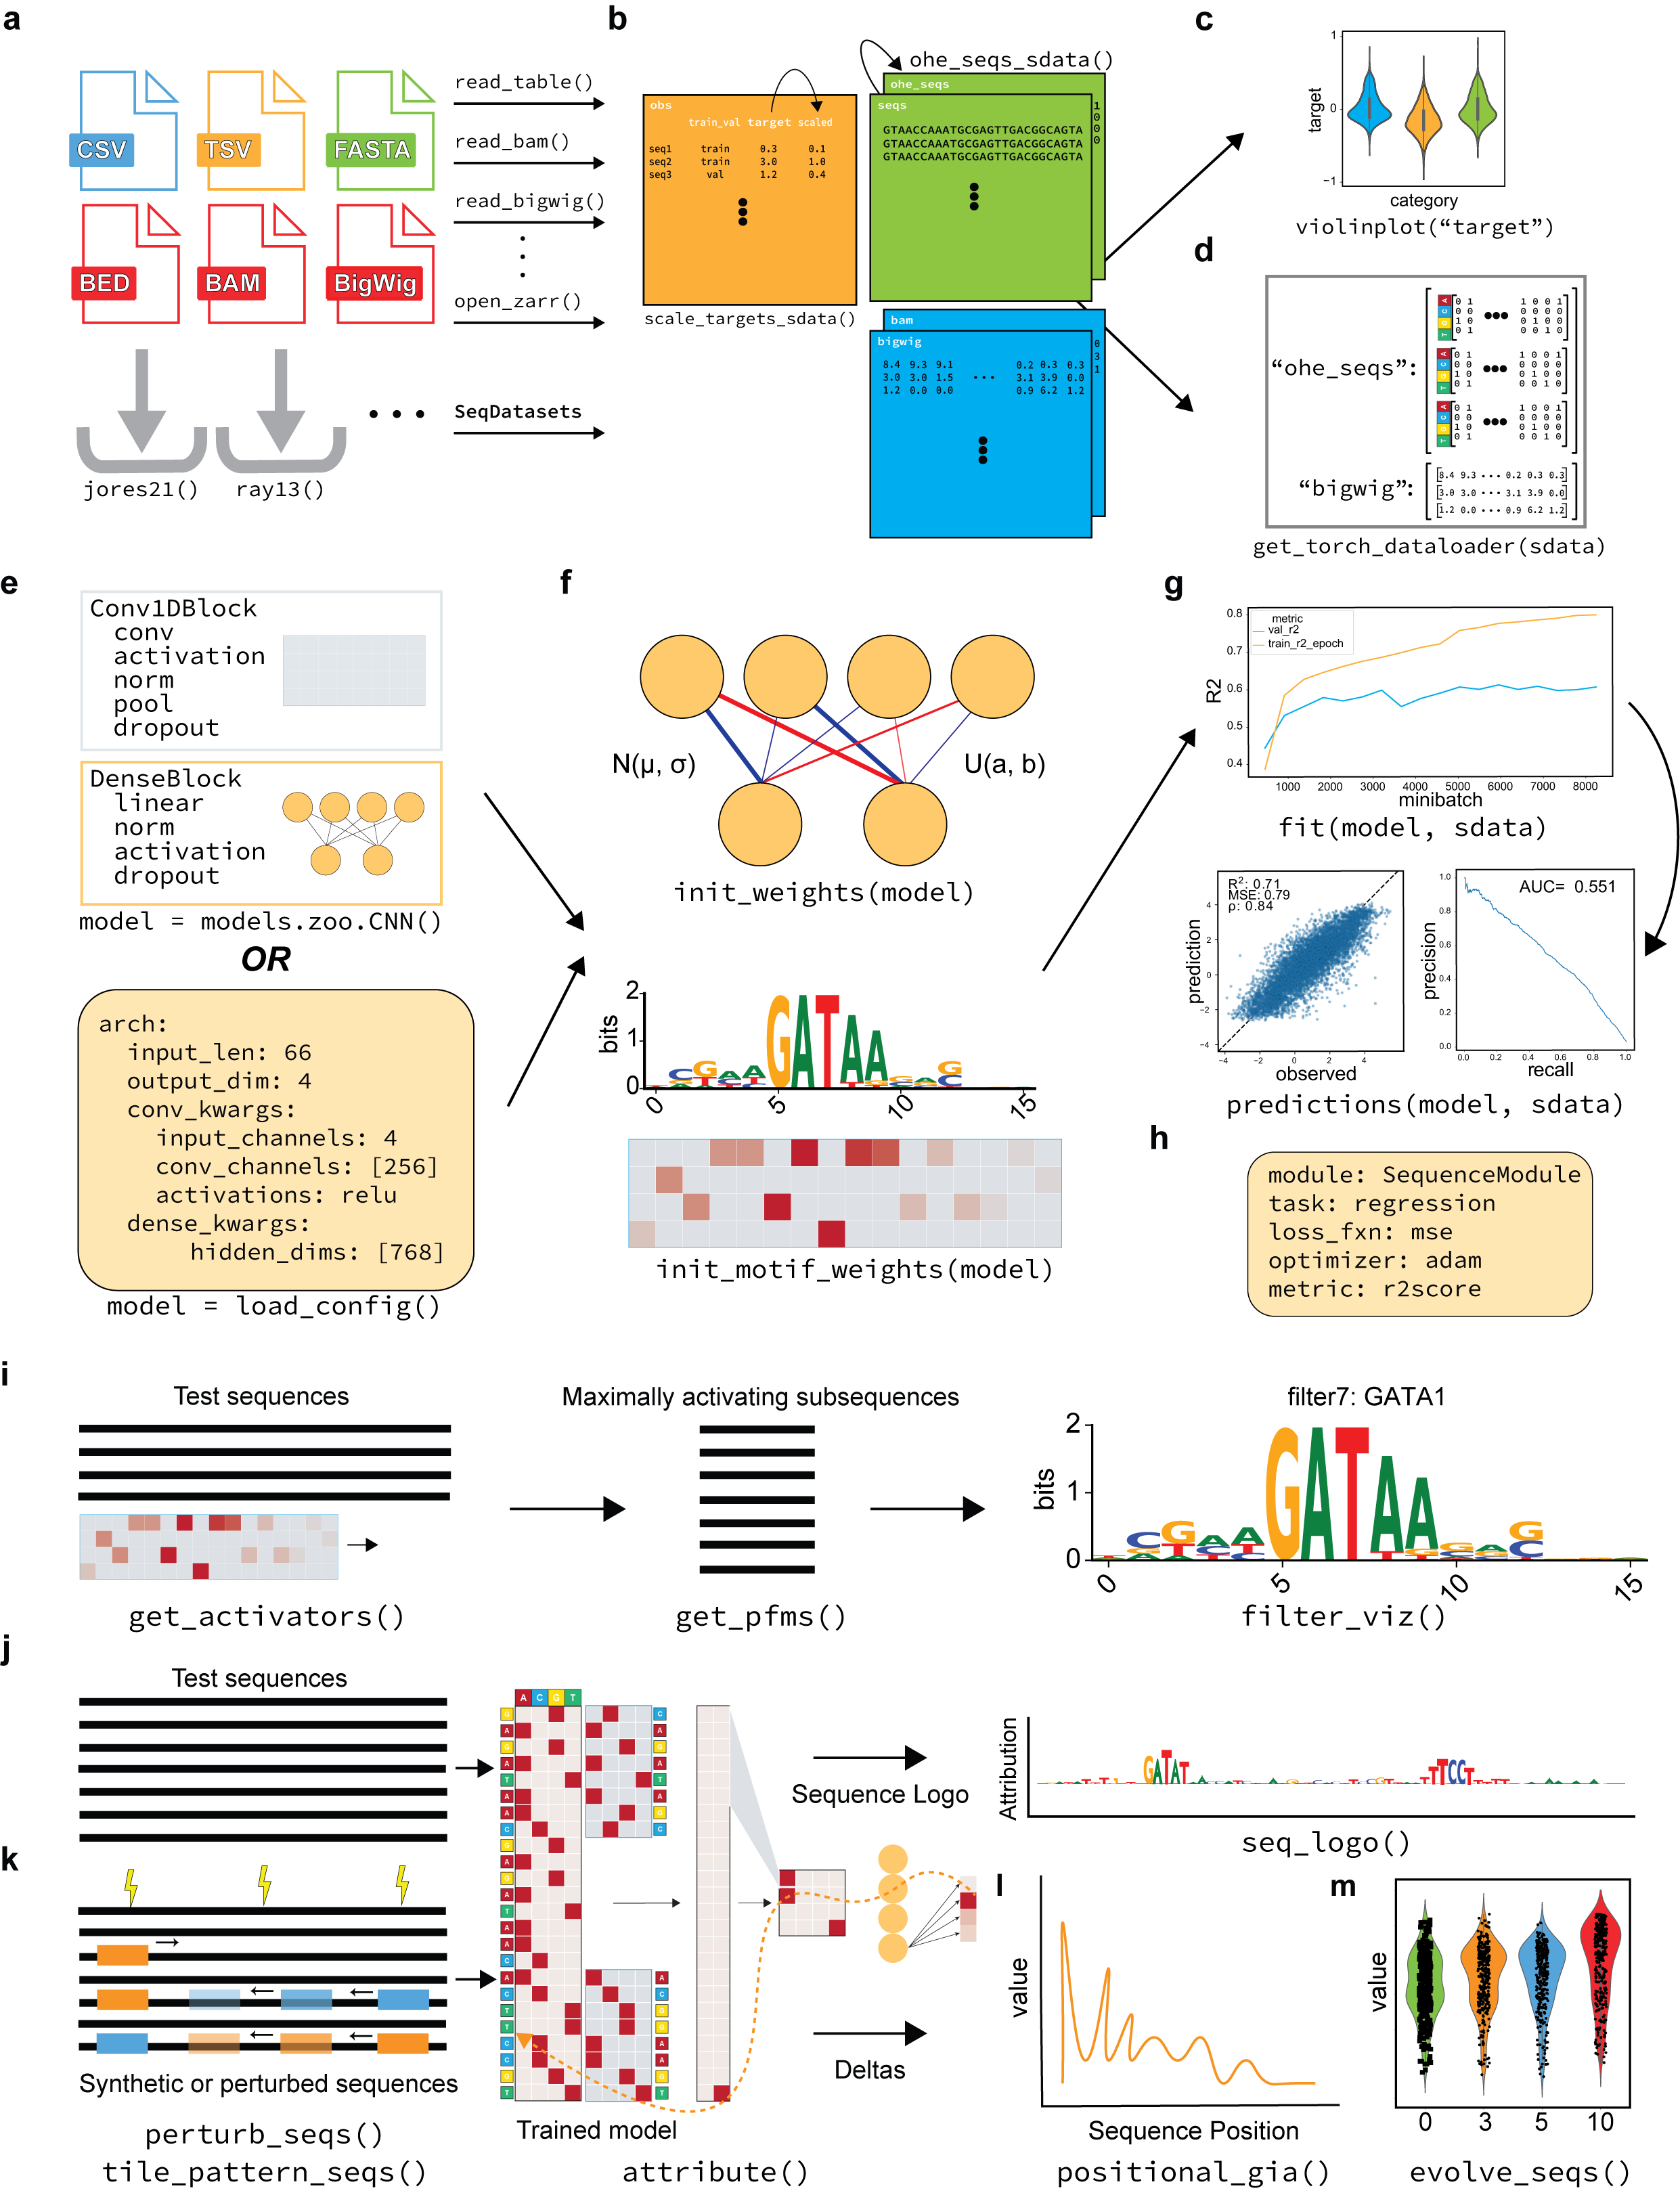
\includegraphics[width=0.9\textwidth, height=0.745\textheight]{1_figures-and-files/extended_data_figure3.png}
    \caption[End-to-end data processing with EUGENe]{\textbf{End-to-end data processing, training, and interpretation with EUGENe}. \textbf{a}, SeqData objects can be loaded from files already on disk, or by calling for a dataset available for download from the SeqDatasets subpackage. Once instantiated, SeqData objects containerize the EUGENe workflow, easing the \textbf{b}, preprocessing of sequences and of sequence metadata, \textbf{c}, the generation of exploratory data analysis plots, and \textbf{d}, the creation of PyTorch loadable datasets and objects. \textbf{e}, An architecture can be instantiated either from a single function call (top) or from a configuration file (bottom). Conv1DBlocks and DenseBlocks both allow for flexibility in the ordering of layers they contain (one example ordering is shown). Instantiated architectures can be \textbf{f}, initialized with a desired initialization scheme, then \textbf{g}, fit to training data and used to predict on held-out data. Performance metric training curves are pictured in the top panel of \textbf{g}, test set performance curves for regression (left) and classification (right) are depicted in the bottom panel of \textbf{g}. Both training and prediction are handled by PyTorch Lightning. We show an example of the arguments for instantiating a SequenceModule in \textbf{h}. \textbf{i}, For filter interpretation, filters in the first convolutional layer are used to scan input sequences for “maximally activating subsequences” that can then be used to generate position frequency matrices and sequence logos. \textbf{j}, Attribution analysis starts by passing inputs sequences through the model to generate an output. This output signal is then backpropagated to the input to generate a per nucleotide score that can be visualized as a sequence logo. \textbf{k}, Random or synthetically designed sequences that have been mutated or have had motifs implanted in them can be scored using a trained model. Results from toy examples of this in silico approach are shown in \textbf{l} and \textbf{m}, which depict a positional importance analysis and a prediction evolution analysis respectively. Example function arguments have been omitted for \textbf{a}, \textbf{b}, \textbf{e}, \textbf{i}, \textbf{j}, \textbf{k}, \textbf{l} and \textbf{m}.}
    \label{fig:5 Figure 5}
\end{figure}

\subsubsection{Data extraction, transformation and loading with SeqData}

The EUGENe workflow begins with extracting data from on-disk formats. Though standardized file formats exist in regulatory genomics, their complexity can make creating model-ready datasets non-trivial. To address this in EUGENe, we created the standalone subpackage SeqData (https://github.com/ML4GLand/SeqData) which flexibly and efficiently reads data from a variety of file formats, including CSV/TSV (tabular), FASTA, BED, BAM, and BigWig (\textbf{Figure~\ref{fig:5 Figure 5}\textbf{a}}, top). The versatility of SeqData enables the generation of many custom datasets from combinations of these file types, including several commonly utilized in regulatory genomics. These include datasets derived from combinations of tabular and FASTA files that are suitable for single and multi-task regression and classification (e.g. DeepSTARR\cite{De_Almeida2022-aa}), datasets from genomic coordinates defined in BED files suitable for multi-task binary classification (e.g. DeepSEA\cite{Zhou2015-rk} or Sei\cite{Chen2022-bn}), and datasets from multiple BigWigs and BED files suitable for binned or base-pair resolution regression (e.g. Basenji\cite{Kelley2018-if} and BPNet\cite{Avsec2021-sw} respectively). EUGENe also supplies a growing collection of hand-curated datasets available via the SeqDatasets subpackage (https://github.com/ML4GLand/SeqDatasets) (\textbf{Supplementary Data~4}) that can be downloaded and subsequently loaded into a workflow via a single function call (\textbf{Figure~\ref{fig:5 Figure 5}\textbf{a}}, bottom).

By default, SeqData reads files from disk as XArray datasets\cite{Hoyer2017-jv} backed by Zarr stores\cite{Miles2023-zk} (\textbf{Figure~\ref{fig:1 Figure 1}\textbf{a}}). We chose to use XArray and Zarr as they are scalable, capable of handling high dimensional data, and have been previously utilized in a variety of bioinformatics domains\cite{Baker2023-sp,Marconato2023-kz,Liu2021-km}. Furthermore, Zarr stores can be loaded out-of-core thanks to functionality offered by XArray and Dask\cite{Team2016-qa}, allowing for processing and training of large-scale datasets (\textbf{Supplementary Figure~\ref{fig:supplementary_4}\textbf{a}}). As is standard in DL, training in EUGENe is always done by loading data into GPU memory in batches (when a GPU is available), but is slowed by using the out-of-core functionality on the CPU (\textbf{Supplementary Figure~\ref{fig:supplementary_4}\textbf{b}}). Thus, the decision on whether to first load the dataset into CPU memory prior to training should balance available resources and dataset size. Certain datasets, such as those used to train Enformer\cite{Avsec2021-hh} or Basenji\cite{Kelley2018-if}, will likely require this out-of-core functionality. However, we have found that many useful and large datasets can entirely fit into memory on machines with less than 32GB of RAM (\textbf{Supplementary Data~5}).

Once created, an array of functions can be called directly on these XArray datasets to perform common preprocessing steps. EUGENe includes a baseline set of functions for train and test set splitting (e.g. by chromosome, fraction, or homology\cite{Teufel2023-kn}) and target normalization (e.g. binning, z-score, clamping, etc.) (\textbf{Figure~\ref{fig:5 Figure 5}\textbf{b}}, left). Sequence preprocessing is handled by the SeqPro subpackage (https://github.com/ML4GLand/SeqPro), which includes Numba accelerated\cite{Lam2015-mo} padding and one-hot encoding of DNA and RNA sequences (\textbf{Figure~\ref{fig:5 Figure 5}\textbf{b}}, right), as well as jittering and k-mer frequency preserving shuffling\cite{Jiang2008-li}. EUGENe also fully supports data visualization through the Matplotlib\cite{Hunter2007-es} and Seaborn\cite{Waskom2021-lk} libraries (\textbf{Figure~\ref{fig:5 Figure 5}\textbf{c}}) and conversion of XArray datasets to formats ingestible by deep learning frameworks in a highly flexible manner (\textbf{Figure~\ref{fig:5 Figure 5}\textbf{d}}). Finally, XArray datasets can easily be converted to more familiar Python data structures (NumPy arrays, Pandas DataFrames, etc.) and back to enable the user to access the functionality of these libraries.

\subsubsection{Model training with PyTorch and PyTorch Lightning}

\subsubsection{Model interpretation with SeqExplainer}

\subsection{Analysis of plant promoter data}

\subsubsection{Data acquisition and preprocessing}

\subsubsection{Model initialization and training}

\subsubsection{Model evaluation and interpretation}

\subsection{Analysis of RNA binding data}

\subsubsection{Data acquisition and preprocessing}

\subsubsection{Model initialization and training}

\subsubsection{Model evaluation}

\subsubsection{Model interpretation}

\subsection{Analysis of JunD binding data}

\subsubsection{Data acquisition and preprocessing}

\subsubsection{Model initialization and training}

\subsubsection{Model evaluation and interpretation}

\subsection{Data visualization software}

\subsection{Statistical methods}

%%%%%%%%%%%%%%%%%%%%%%%%%%%%%%%%%%%%%%%%%%%%%%%%%%%%%%%%%%%%%%%%%%%%%%%%%%%%%%%%
\section{Data availability}
%%%%%%%%%%%%%%%%%%%%%%%%%%%%%%%%%%%%%%%%%%%%%%%%%%%%%%%%%%%%%%%%%%%%%%%%%%%%%%%%

%%%%%%%%%%%%%%%%%%%%%%%%%%%%%%%%%%%%%%%%%%%%%%%%%%%%%%%%%%%%%%%%%%%%%%%%%%%%%%%%
\section{Code availability}
%%%%%%%%%%%%%%%%%%%%%%%%%%%%%%%%%%%%%%%%%%%%%%%%%%%%%%%%%%%%%%%%%%%%%%%%%%%%%%%%

%%%%%%%%%%%%%%%%%%%%%%%%%%%%%%%%%%%%%%%%%%%%%%%%%%%%%%%%%%%%%%%%%%%%%%%%%%%%%%%%
\section{Acknowledgements}
%%%%%%%%%%%%%%%%%%%%%%%%%%%%%%%%%%%%%%%%%%%%%%%%%%%%%%%%%%%%%%%%%%%%%%%%%%%%%%%%

%%%%%%%%%%%%%%%%%%%%%%%%%%%%%%%%%%%%%%%%%%%%%%%%%%%%%%%%%%%%%%%%%%%%%%%%%%%%%%%%
\section{Author information}
%%%%%%%%%%%%%%%%%%%%%%%%%%%%%%%%%%%%%%%%%%%%%%%%%%%%%%%%%%%%%%%%%%%%%%%%%%%%%%%%

%%%%%%%%%%%%%%%%%%%%%%%%%%%%%%%%%%%%%%%%%%%%%%%%%%%%%%%%%%%%%%%%%%%%%%%%%%%%%%%%
\section{Ethics declarations}
%%%%%%%%%%%%%%%%%%%%%%%%%%%%%%%%%%%%%%%%%%%%%%%%%%%%%%%%%%%%%%%%%%%%%%%%%%%%%%%%

\subsection{Competing interests}
